\chapter{Father and Son}

M. Noirtier—for it was, indeed, he who entered—looked after the servant
until the door was closed, and then, fearing, no doubt, that he might
be overheard in the antechamber, he opened the door again, nor was the
precaution useless, as appeared from the rapid retreat of Germain, who
proved that he was not exempt from the sin which ruined our first
parents. M. Noirtier then took the trouble to close and bolt the
antechamber door, then that of the bedchamber, and then extended his
hand to Villefort, who had followed all his motions with surprise which
he could not conceal.

“Well, now, my dear Gérard,” said he to the young man, with a very
significant look, “do you know, you seem as if you were not very glad
to see me?”

“My dear father,” said Villefort, “I am, on the contrary, delighted;
but I so little expected your visit, that it has somewhat overcome me.”

“But, my dear fellow,” replied M. Noirtier, seating himself, “I might
say the same thing to you, when you announce to me your wedding for the
28th of February, and on the 3rd of March you turn up here in Paris.”

“And if I have come, my dear father,” said Gérard, drawing closer to M.
Noirtier, “do not complain, for it is for you that I came, and my
journey will be your salvation.”

“Ah, indeed!” said M. Noirtier, stretching himself out at his ease in
the chair. “Really, pray tell me all about it, for it must be
interesting.”

“Father, you have heard speak of a certain Bonapartist club in the Rue
Saint-Jacques?”

“No. 53; yes, I am vice-president.”

“Father, your coolness makes me shudder.”

“Why, my dear boy, when a man has been proscribed by the mountaineers,
has escaped from Paris in a hay-cart, been hunted over the plains of
Bordeaux by Robespierre’s bloodhounds, he becomes accustomed to most
things. But go on, what about the club in the Rue Saint-Jacques?”

“Why, they induced General Quesnel to go there, and General Quesnel,
who quitted his own house at nine o’clock in the evening, was found the
next day in the Seine.”

\begin{figure}[ht]
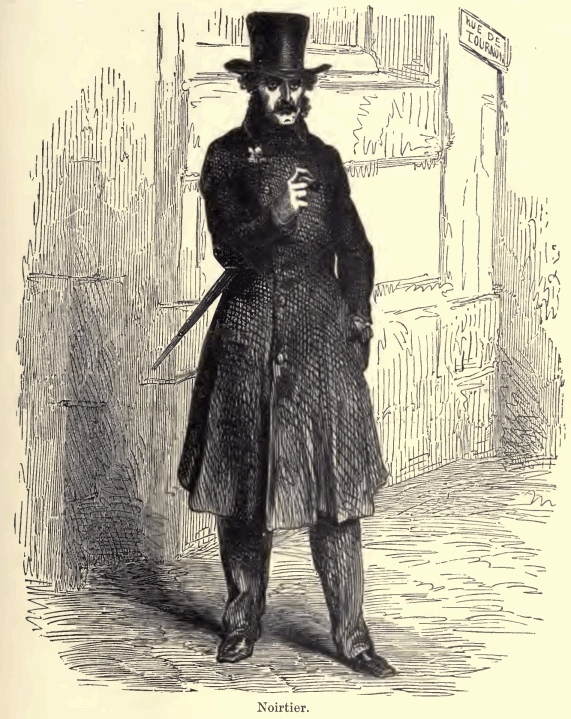
\includegraphics[width=\textwidth]{0151m.jpg}
\end{figure}

“And who told you this fine story?”

“The king himself.”

“Well, then, in return for your story,” continued Noirtier, “I will
tell you another.”

“My dear father, I think I already know what you are about to tell me.”

“Ah, you have heard of the landing of the emperor?”

“Not so loud, father, I entreat of you—for your own sake as well as
mine. Yes, I heard this news, and knew it even before you could; for
three days ago I posted from Marseilles to Paris with all possible
speed, half-desperate at the enforced delay.”

“Three days ago? You are crazy. Why, three days ago the emperor had not
landed.”

“No matter, I was aware of his intention.”

“How did you know about it?”

“By a letter addressed to you from the Island of Elba.”

“To me?”

“To you; and which I discovered in the pocket-book of the messenger.
Had that letter fallen into the hands of another, you, my dear father,
would probably ere this have been shot.” Villefort’s father laughed.

“Come, come,” said he, “will the Restoration adopt imperial methods so
promptly? Shot, my dear boy? What an idea! Where is the letter you
speak of? I know you too well to suppose you would allow such a thing
to pass you.”

“I burnt it, for fear that even a fragment should remain; for that
letter must have led to your condemnation.”

“And the destruction of your future prospects,” replied Noirtier; “yes,
I can easily comprehend that. But I have nothing to fear while I have
you to protect me.”

“I do better than that, sir—I save you.”

“You do? Why, really, the thing becomes more and more dramatic—explain
yourself.”

“I must refer again to the club in the Rue Saint-Jacques.”

“It appears that this club is rather a bore to the police. Why didn’t
they search more vigilantly? they would have found——”

“They have not found; but they are on the track.”

“Yes, that the usual phrase; I am quite familiar with it. When the
police is at fault, it declares that it is on the track; and the
government patiently awaits the day when it comes to say, with a
sneaking air, that the track is lost.”

“Yes, but they have found a corpse; the general has been killed, and in
all countries they call that a murder.”

“A murder do you call it? why, there is nothing to prove that the
general was murdered. People are found every day in the Seine, having
thrown themselves in, or having been drowned from not knowing how to
swim.”

“Father, you know very well that the general was not a man to drown
himself in despair, and people do not bathe in the Seine in the month
of January. No, no, do not be deceived; this was murder in every sense
of the word.”

“And who thus designated it?”

“The king himself.”

“The king! I thought he was philosopher enough to allow that there was
no murder in politics. In politics, my dear fellow, you know, as well
as I do, there are no men, but ideas—no feelings, but interests; in
politics we do not kill a man, we only remove an obstacle, that is all.
Would you like to know how matters have progressed? Well, I will tell
you. It was thought reliance might be placed in General Quesnel; he was
recommended to us from the Island of Elba; one of us went to him, and
invited him to the Rue Saint-Jacques, where he would find some friends.
He came there, and the plan was unfolded to him for leaving Elba, the
projected landing, etc. When he had heard and comprehended all to the
fullest extent, he replied that he was a royalist. Then all looked at
each other,—he was made to take an oath, and did so, but with such an
ill grace that it was really tempting Providence to swear thus, and
yet, in spite of that, the general was allowed to depart free—perfectly
free. Yet he did not return home. What could that mean? why, my dear
fellow, that on leaving us he lost his way, that’s all. A murder?
really, Villefort, you surprise me. You, a deputy procureur, to found
an accusation on such bad premises! Did I ever say to you, when you
were fulfilling your character as a royalist, and cut off the head of
one of my party, ‘My son, you have committed a murder?’ No, I said,
‘Very well, sir, you have gained the victory; tomorrow, perchance, it
will be our turn.’”

“But, father, take care; when our turn comes, our revenge will be
sweeping.”

“I do not understand you.”

“You rely on the usurper’s return?”

“We do.”

“You are mistaken; he will not advance two leagues into the interior of
France without being followed, tracked, and caught like a wild beast.”

“My dear fellow, the emperor is at this moment on the way to Grenoble;
on the 10th or 12th he will be at Lyons, and on the 20th or 25th at
Paris.”

“The people will rise.”

“Yes, to go and meet him.”

“He has but a handful of men with him, and armies will be despatched
against him.”

“Yes, to escort him into the capital. Really, my dear Gérard, you are
but a child; you think yourself well informed because the telegraph has
told you, three days after the landing, ‘The usurper has landed at
Cannes with several men. He is pursued.’ But where is he? what is he
doing? You do not know at all, and in this way they will chase him to
Paris, without drawing a trigger.”

“Grenoble and Lyons are faithful cities, and will oppose to him an
impassable barrier.”

“Grenoble will open her gates to him with enthusiasm—all Lyons will
hasten to welcome him. Believe me, we are as well informed as you, and
our police are as good as your own. Would you like a proof of it? well,
you wished to conceal your journey from me, and yet I knew of your
arrival half an hour after you had passed the barrier. You gave your
direction to no one but your postilion, yet I have your address, and in
proof I am here the very instant you are going to sit at table. Ring,
then, if you please, for a second knife, fork, and plate, and we will
dine together.”

“Indeed!” replied Villefort, looking at his father with astonishment,
“you really do seem very well informed.”

“Eh? the thing is simple enough. You who are in power have only the
means that money produces—we who are in expectation, have those which
devotion prompts.”

“Devotion!” said Villefort, with a sneer.

“Yes, devotion; for that is, I believe, the phrase for hopeful
ambition.”

And Villefort’s father extended his hand to the bell-rope, to summon
the servant whom his son had not called. Villefort caught his arm.

“Wait, my dear father,” said the young man, “one word more.”

“Say on.”

“However stupid the royalist police may be, they do know one terrible
thing.”

“What is that?”

“The description of the man who, on the morning of the day when General
Quesnel disappeared, presented himself at his house.”

“Oh, the admirable police have found that out, have they? And what may
be that description?”

“Dark complexion; hair, eyebrows, and whiskers black; blue frock-coat,
buttoned up to the chin; rosette of an officer of the Legion of Honor
in his button-hole; a hat with wide brim, and a cane.”

“Ah, ha, that’s it, is it?” said Noirtier; “and why, then, have they
not laid hands on him?”

“Because yesterday, or the day before, they lost sight of him at the
corner of the Rue Coq-Héron.”

“Didn’t I say that your police were good for nothing?”

“Yes; but they may catch him yet.”

“True,” said Noirtier, looking carelessly around him, “true, if this
person were not on his guard, as he is;” and he added with a smile, “He
will consequently make a few changes in his personal appearance.” At
these words he rose, and put off his frock-coat and cravat, went
towards a table on which lay his son’s toilet articles, lathered his
face, took a razor, and, with a firm hand, cut off the compromising
whiskers. Villefort watched him with alarm not devoid of admiration.

His whiskers cut off, Noirtier gave another turn to his hair; took,
instead of his black cravat, a colored neckerchief which lay at the top
of an open portmanteau; put on, in lieu of his blue and high-buttoned
frock-coat, a coat of Villefort’s of dark brown, and cut away in front;
tried on before the glass a narrow-brimmed hat of his son’s, which
appeared to fit him perfectly, and, leaving his cane in the corner
where he had deposited it, he took up a small bamboo switch, cut the
air with it once or twice, and walked about with that easy swagger
which was one of his principal characteristics.

“Well,” he said, turning towards his wondering son, when this disguise
was completed, “well, do you think your police will recognize me now.”

“No, father,” stammered Villefort; “at least, I hope not.”

“And now, my dear boy,” continued Noirtier, “I rely on your prudence to
remove all the things which I leave in your care.”

“Oh, rely on me,” said Villefort.

“Yes, yes; and now I believe you are right, and that you have really
saved my life; be assured I will return the favor hereafter.”

Villefort shook his head.

“You are not convinced yet?”

“I hope at least, that you may be mistaken.”

“Shall you see the king again?”

“Perhaps.”

“Would you pass in his eyes for a prophet?”

“Prophets of evil are not in favor at the court, father.”

“True, but some day they do them justice; and supposing a second
restoration, you would then pass for a great man.”

“Well, what should I say to the king?”

“Say this to him: ‘Sire, you are deceived as to the feeling in France,
as to the opinions of the towns, and the prejudices of the army; he
whom in Paris you call the Corsican ogre, who at Nevers is styled the
usurper, is already saluted as Bonaparte at Lyons, and emperor at
Grenoble. You think he is tracked, pursued, captured; he is advancing
as rapidly as his own eagles. The soldiers you believe to be dying with
hunger, worn out with fatigue, ready to desert, gather like atoms of
snow about the rolling ball as it hastens onward. Sire, go, leave
France to its real master, to him who acquired it, not by purchase, but
by right of conquest; go, sire, not that you incur any risk, for your
adversary is powerful enough to show you mercy, but because it would be
humiliating for a grandson of Saint Louis to owe his life to the man of
Arcola, Marengo, Austerlitz.’ Tell him this, Gérard; or, rather, tell
him nothing. Keep your journey a secret; do not boast of what you have
come to Paris to do, or have done; return with all speed; enter
Marseilles at night, and your house by the back-door, and there remain,
quiet, submissive, secret, and, above all, inoffensive; for this time,
I swear to you, we shall act like powerful men who know their enemies.
Go, my son—go, my dear Gérard, and by your obedience to my paternal
orders, or, if you prefer it, friendly counsels, we will keep you in
your place. This will be,” added Noirtier, with a smile, “one means by
which you may a second time save me, if the political balance should
some day take another turn, and cast you aloft while hurling me down.
Adieu, my dear Gérard, and at your next journey alight at my door.”

Noirtier left the room when he had finished, with the same calmness
that had characterized him during the whole of this remarkable and
trying conversation. Villefort, pale and agitated, ran to the window,
put aside the curtain, and saw him pass, cool and collected, by two or
three ill-looking men at the corner of the street, who were there,
perhaps, to arrest a man with black whiskers, and a blue frock-coat,
and hat with broad brim.

Villefort stood watching, breathless, until his father had disappeared
at the Rue Bussy. Then he turned to the various articles he had left
behind him, put the black cravat and blue frock-coat at the bottom of
the portmanteau, threw the hat into a dark closet, broke the cane into
small bits and flung it in the fire, put on his travelling-cap, and
calling his valet, checked with a look the thousand questions he was
ready to ask, paid his bill, sprang into his carriage, which was ready,
learned at Lyons that Bonaparte had entered Grenoble, and in the midst
of the tumult which prevailed along the road, at length reached
Marseilles, a prey to all the hopes and fears which enter into the
heart of man with ambition and its first successes.
